%% LyX 2.4.3 created this file.  For more info, see https://www.lyx.org/.
%% Do not edit unless you really know what you are doing.
\documentclass[11pt,oneside,czech,american]{book}
\usepackage[T1]{fontenc}
\usepackage[utf8]{inputenc}
\setcounter{secnumdepth}{3}
\usepackage{url}
\usepackage{amsmath}
\usepackage{amsthm}

\usepackage[svgnames]{xcolor}
\usepackage{graphicx}
\usepackage{minted}
\usemintedstyle{default}
\setminted{
    frame=lines,
    framesep=2mm,
    breaklines=true,
    bgcolor=gray!10
}
\usepackage[a4paper]{geometry}
\geometry{verbose,tmargin=4cm,bmargin=3cm,lmargin=3cm,rmargin=2.5cm,headheight=0.8cm,headsep=1cm,footskip=0.5cm}

\usepackage{setspace}


%%%%%%%%%%%%%%%%%%%%%%%%%%%%%% Textclass specific LaTeX commands.
\newenvironment{lyxlist}[1]
{\begin{list}{}
{\settowidth{\labelwidth}{#1}
\setlength{\leftmargin}{\labelwidth}
\addtolength{\leftmargin}{\labelsep}
\renewcommand{\makelabel}[1]{##1\hfil}}}
{\end{list}}

%%%%%%%%%%%%%%%%%%%%%%%%%%%%%% User specified LaTeX commands.
%% Font setup: please leave the LyX font settings all set to 'default'
%% if you want to use any of these packages:

%% Use Times New Roman font for text and Belleek font for math
%% Please make sure that the 'esint' package is turned off in the
%% 'Math options' page.
\usepackage[varg]{txfonts}

%% Use Utopia text with Fourier-GUTenberg math
%\usepackage{fourier}

%% Bitstream Charter text with Math Design math
%\usepackage[charter]{mathdesign}

%%---------------------------------------------------------------------

%% Make the multiline figure/table captions indent so that the second
%% line "hangs" right below the first one.
%\usepackage[format=hang]{caption}

%% Indent even the first paragraph in each section
\usepackage{indentfirst}

%%---------------------------------------------------------------------

\usepackage{pdfpages}

%%---------------------------------------------------------------------

%% Disable page numbers in the TOC. LOF, LOT (TOC automatically
%% adds \thispagestyle{chapter} if not overriden
%\addtocontents{toc}{\protect\thispagestyle{empty}}
%\addtocontents{lof}{\protect\thispagestyle{empty}}
%\addtocontents{lot}{\protect\thispagestyle{empty}}

%% Shifts the top line of the TOC (not the title) 1cm upwards
%% so that the whole TOC fits on 1 page. Additional page size
%% adjustment is performed at the point where the TOC
%% is inserted.
%\addtocontents{toc}{\protect\vspace{-1cm}}

%%---------------------------------------------------------------------

% completely avoid orphans (first lines of a new paragraph on the bottom of a page)
\clubpenalty=9500

% completely avoid widows (last lines of paragraph on a new page)
\widowpenalty=9500

% disable hyphenation of acronyms
\hyphenation{CDFA HARDI HiPPIES IKEM InterTrack MEGIDDO MIMD MPFA DICOM ASCLEPIOS MedInria}

%%---------------------------------------------------------------------

%% Print out all vectors in bold type instead of printing an arrow above them
\renewcommand{\vec}[1]{\boldsymbol{#1}}

% Replace standard \cite by the parenthetical variant \citep
%\renewcommand{\cite}{\citep}


\usepackage{biblatex}
\usepackage{babel}
\usepackage{hyperref}
\usepackage{color}
\usepackage{multirow}
\addbibresource{export.bib}

\begin{document}
    \newcommand{\documentdate}{August 4, 2025}

%%\def\documentdate{\today}

    \pagestyle{empty}
    {\centering

    \noindent{}%
        \begin{minipage}[c]{3cm}%
            \begin{center}
                
\includegraphics[width=3cm,keepaspectratio,height=3cm]{Images/TITLE/cvut}

            \end{center}%
        \end{minipage}%
        \begin{minipage}[c]{0.6\linewidth}%
            \begin{center}
            {\large\textsc{Czech Technical University in Prague}}{\large}
                \\
                {\large Faculty of Nuclear Sciences and Physical Engineering}

            \end{center}%
        \end{minipage}%
        \begin{minipage}[c]{3cm}%
            \begin{center}
                
\includegraphics[width=3cm,keepaspectratio,height=3cm]{Images/TITLE/fjfi}

            \end{center}%
        \end{minipage}

        \vspace{3cm}

        {\huge\textbf{Web application for team work organization}}{\huge\par}

        \vspace{1cm}

        \selectlanguage{czech}%
        {\huge\textbf{Webová aplikace pro organizaci týmové práce}}{\huge\par}

        \selectlanguage{american}%
        \vspace{2cm}

        {\large Bachelor's Degree Project}{\large\par}

    }

    \vfill{}

    \begin{lyxlist}{MMMMMMMMM}
        \begin{singlespace}
            \item [{Author:}] \textbf{Kirill Borodinskiy}
            \item [{Supervisor:}] \textbf{doc. Ing. Miroslav Virius, CSc.}
            \item [{Academic~year:}] 2024/2025
        \end{singlespace}
    \end{lyxlist}

    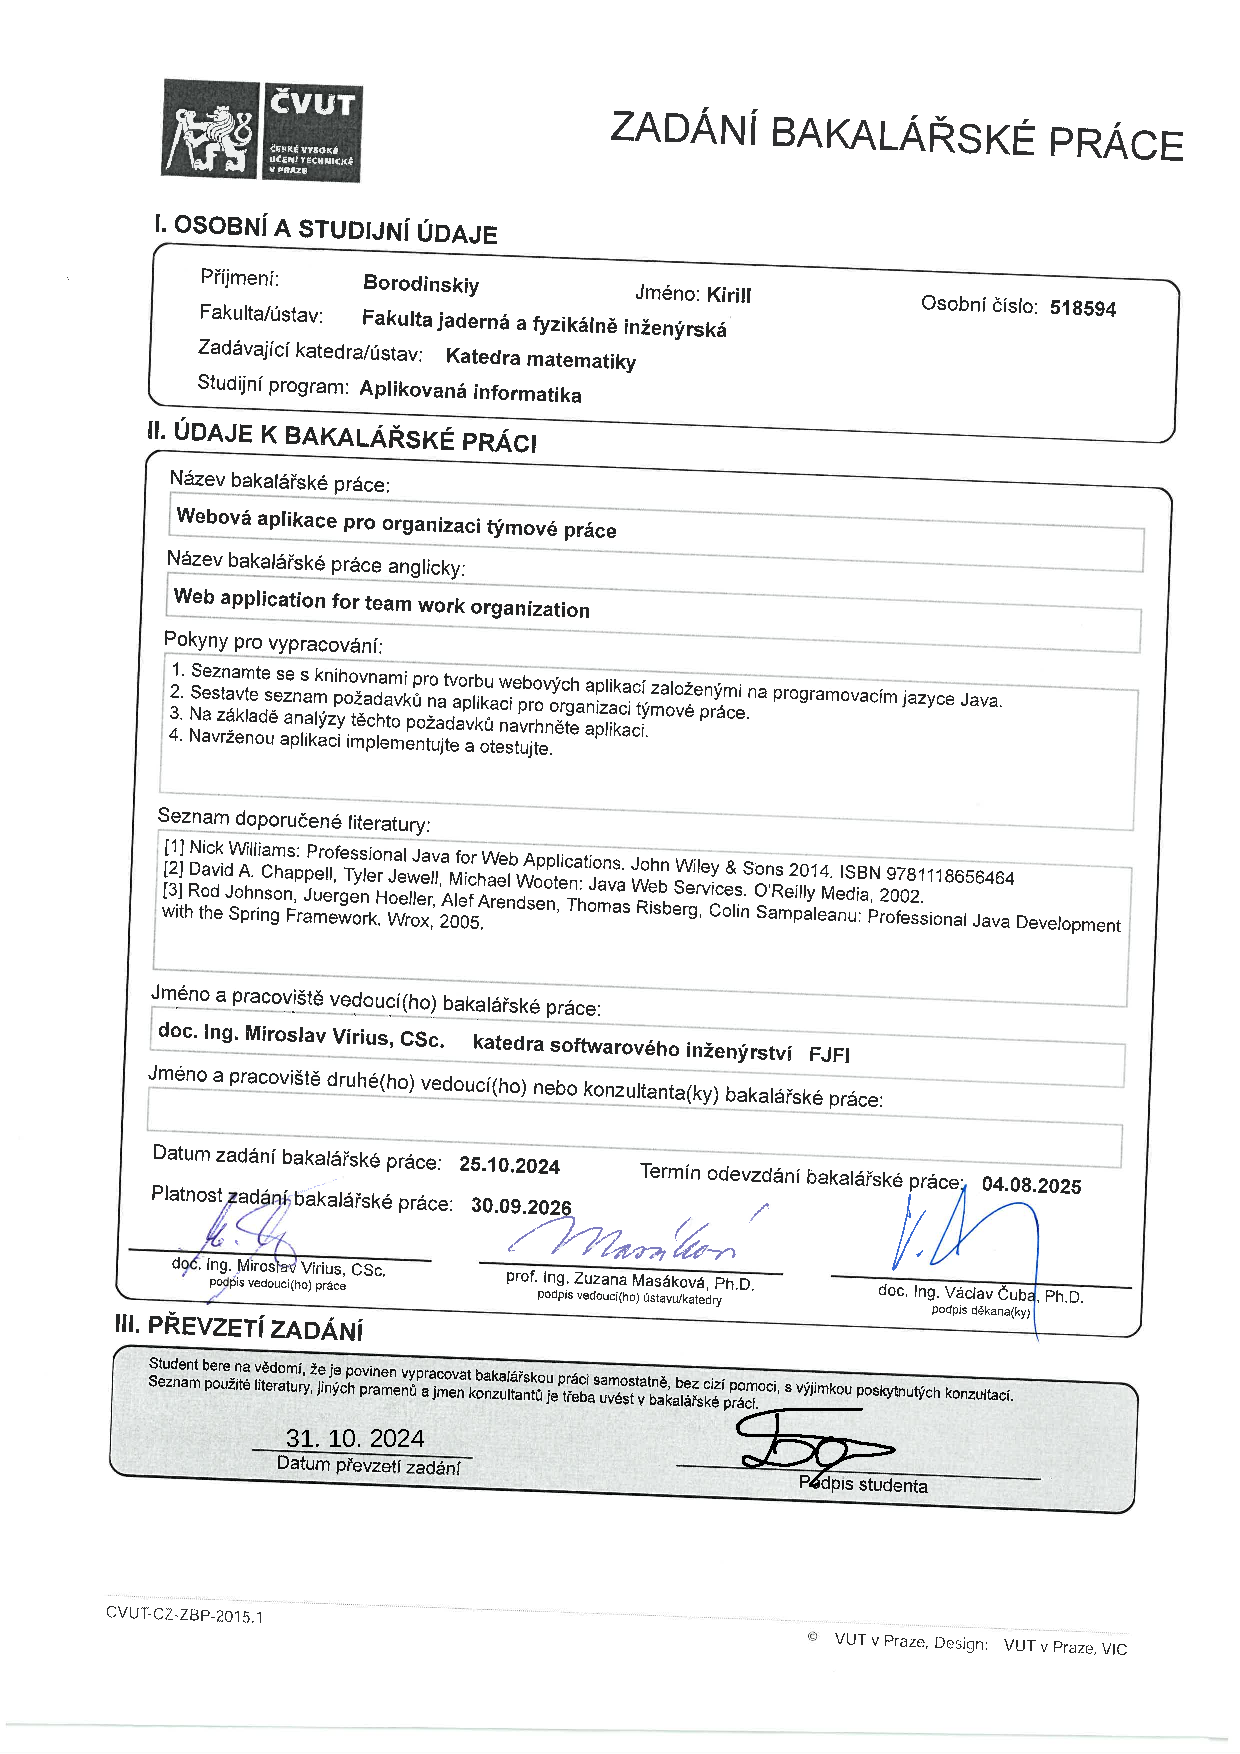
\includepdf[]{BPZADANI.pdf}
    
\includepdf[]{document_24_filename.pdf}

    \noindent{\Large\emph{Acknowledgment:}}{\Large\par}

    \noindent I would like to thank my mother Elena and my girlfriend Anastasiia for their moral support.
    I would like to thank my supervisor, Miroslav Virius, for their help in organization of my bachelor's thesis project.

    \vfill

    \noindent{\Large\emph{Author's declaration:}}{\Large\par}

    \noindent I declare that this Bachelor's Degree Project is entirely
    my own work and I have listed all the used sources in the bibliography.
    AI tools were used in full accordance with the guidelines established
    by CTU in Prague.

    \bigskip{}

    \noindent Prague, \documentdate\hfill{}Kirill Borodinskiy

    \vspace{2cm}

    \newpage{}

    \selectlanguage{czech}%
    \begin{onehalfspace}
        \noindent\emph{Název práce:}

        \noindent\textbf{Webová aplikace pro organizaci týmové práce}
    \end{onehalfspace}

    \bigskip{}

    \noindent\emph{Autor:} Kirill Borodinskiy

    \bigskip{}

    \noindent\emph{Studijní program:}
    \bigskip{} Aplikovaná informatika


    \bigskip{}

    \noindent\emph{Druh práce:} Bakalářská práce

    \bigskip{}

    \noindent\emph{Vedoucí práce:}doc.
    Ing.
    Miroslav Virius, CSc., DrSc.,
    ČVUT,Fakulta jaderná a fyzikálně inženýrská, Katedra softwarového inženýrství



    \bigskip{}

    \bigskip{}

    \noindent\emph{Abstrakt:} Tato práce představuje návrh a implementaci TeamJob, samostatně hostovaného open-source systému pro plánování týmové práce určeného pro organizace, které upřednostňují soukromí, flexibilitu a kontrolu nad svými plánovacími daty.
    Aplikace je postavena pomocí moderních Java webových technologií včetně Spring Boot, Thymeleaf a PostgreSQL s implementací modulární MVC architektury a JWT autentifikací pro zajištění bezpečných bezstavových uživatelských relací.
    Systém poskytuje komplexní možnosti správy událostí včetně detekce konfliktů, pokročilého filtrování podle uživatelů, místností a štítků a flexibilního systému štítkování pro organizační účely.
    Implementace zahrnuje řízení přístupu na základě rolí, auditní stopy a funkce optimalizace zdrojů prostřednictvím funkce ``Find Available''.
    Rozsáhlé testování na úrovni služeb, kontrolerů a repozitářů potvrdilo spolehlivost systému s 100\% úspěšností testů napříč 47 testovacími případy.
    Zatímco backendová logika pro opakující se události je plně implementována, frontendové zobrazení vyžaduje další vývoj.
    Projekt demonstruje proveditelnost vytvoření přizpůsobitelné, soukromí zaměřené plánovací platformy, která vyvažuje funkcionalitu s bezpečností a poskytuje solidní základ pro budoucí vylepšení v kolaborativních plánovacích systémech.

    \bigskip{}

    \noindent\emph{Klíčová slova:} kalendářový systém, JWT autentifikace, Java, PostgreSQL, Spring Boot, správa událostí, týmová spolupráce, webová aplikace

    \newpage
    \selectlanguage{american}%
    \vfill{}
    ~

    \begin{onehalfspace}
        \noindent\emph{Title:}

        \noindent\textbf{Web application for team work organization}
    \end{onehalfspace}

    \bigskip{}

    \noindent\emph{Author:} Kirill Borodinskiy

    \bigskip{}

    \noindent\emph{Abstract:} This thesis explains the design and implementation of TeamJob, a self-hosted, open-source team scheduling system developed for organizations that prioritize privacy, flexibility, and control over their scheduling data.
    The application is built using modern Java web technologies, including Spring Boot, Thymeleaf, and PostgreSQL. It features a modular MVC architecture with JWT-based authentication to ensure secure, stateless user sessions.
    The system provides comprehensive event management capabilities, such as conflict detection and advanced filtering by users, rooms, and tags, along with a versatile tagging system tailored for organizational purposes.
    The implementation includes role-based access control, audit trails, and resource optimization functionalities executed through the ``Find Available'' feature.
    Extensive testing conducted at the service, controller, and repository levels verified the system's reliability, yielding a test pass rate of 100\% across 47 test cases.
    The back-end logic for recurring events has been entirely implemented, but further enhancement of the front-end display is required.
    This project demonstrates the feasibility of developing a customizable, privacy-centric scheduling platform that proficiently integrates functionality with security, thus providing a solid foundation for future advancements in collaborative scheduling systems.
    \bigskip{}

    \noindent\emph{Key words:} calendar system, event management, JWT authentication, PostgreSQL, Spring Boot, Java, resource scheduling, role-based access control, team collaboration, web application

    \newpage{}

    \pagestyle{plain}

    \tableofcontents{}

    \newpage{}


    \chapter{Introduction}\label{ch:introduction}
    \section*{Motivation}
Efficient team schedule planning is a complex challenge, particularly in organizations that require real-time coordination and resource management.
Existing scheduling services often have significant limitations, such as proprietary nature, lack of customization, and dependence on third-party infrastructure.
This project aims to develop a self-hosted open-source booking system designed for organizations that need a private, adaptable scheduling solution.
The system will provide a web-based interface where users can:
\begin{itemize}
    \item Make and manage reservations
    \item Check real-time room availability
    \item  Filter bookings by person or room
    \item View all reservations on a centralized calendar
\end{itemize}

The backend will be built using the Spring Framework, ensuring scalability, security, and ease of integration with existing infrastructure.
Unlike cloud-based alternatives, this system will store all data locally, giving organizations complete privacy and control over scheduling information.
By combining flexibility, transparency, and data privacy, this project can provide a practical alternative to commercial scheduling tools, empowering organizations with greater autonomy and customization options.
\addcontentsline{toc}{section}{Motivation}


\pagestyle{headings}
Here we will talk about why the calendar is needed

Firstly, lets take a look at the current solution used by my university,CTU. Rozvrh.fjfi.cvut.cz is a website where students can see their schedule.
\section{The current solution}\label{sec:the-current-solution}
\begin{figure}[h]
  \centering
  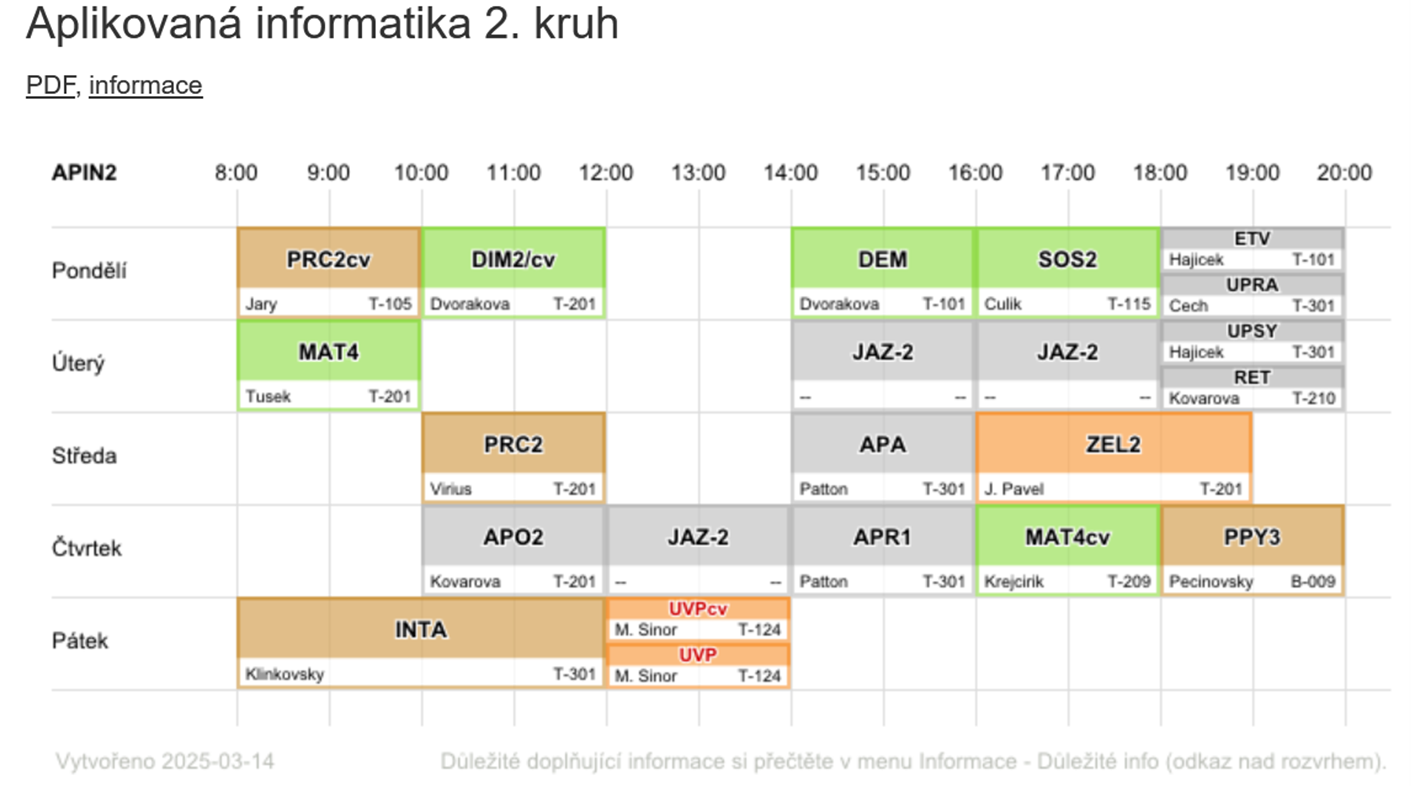
\includegraphics[width=0.6\textwidth]{img}
  \caption{Screenshot of the current solution}
  \label{fig:rozvrh}
\end{figure}

It can be seen on~\ref{fig:rozvrh} that while the website completes its main purpose, it is not customizable, which makes it hard to use.
For example, if a student has a class that is from another year or/and program, they have to look at another picture and manually compare them.
From my experience, many students have screenshots on their phones and they cross-out the classes that they are not registered to.
They may have a few screenshots, for different programs or years.
It is not a good solution, as it allows for misunderstandings and mistakes.

This is why a project focused on creating a calendar that is easy to use and customizable is needed.
\section{The solution}\label{sec:the-solution}
\begin{figure}[h]
  \centering
  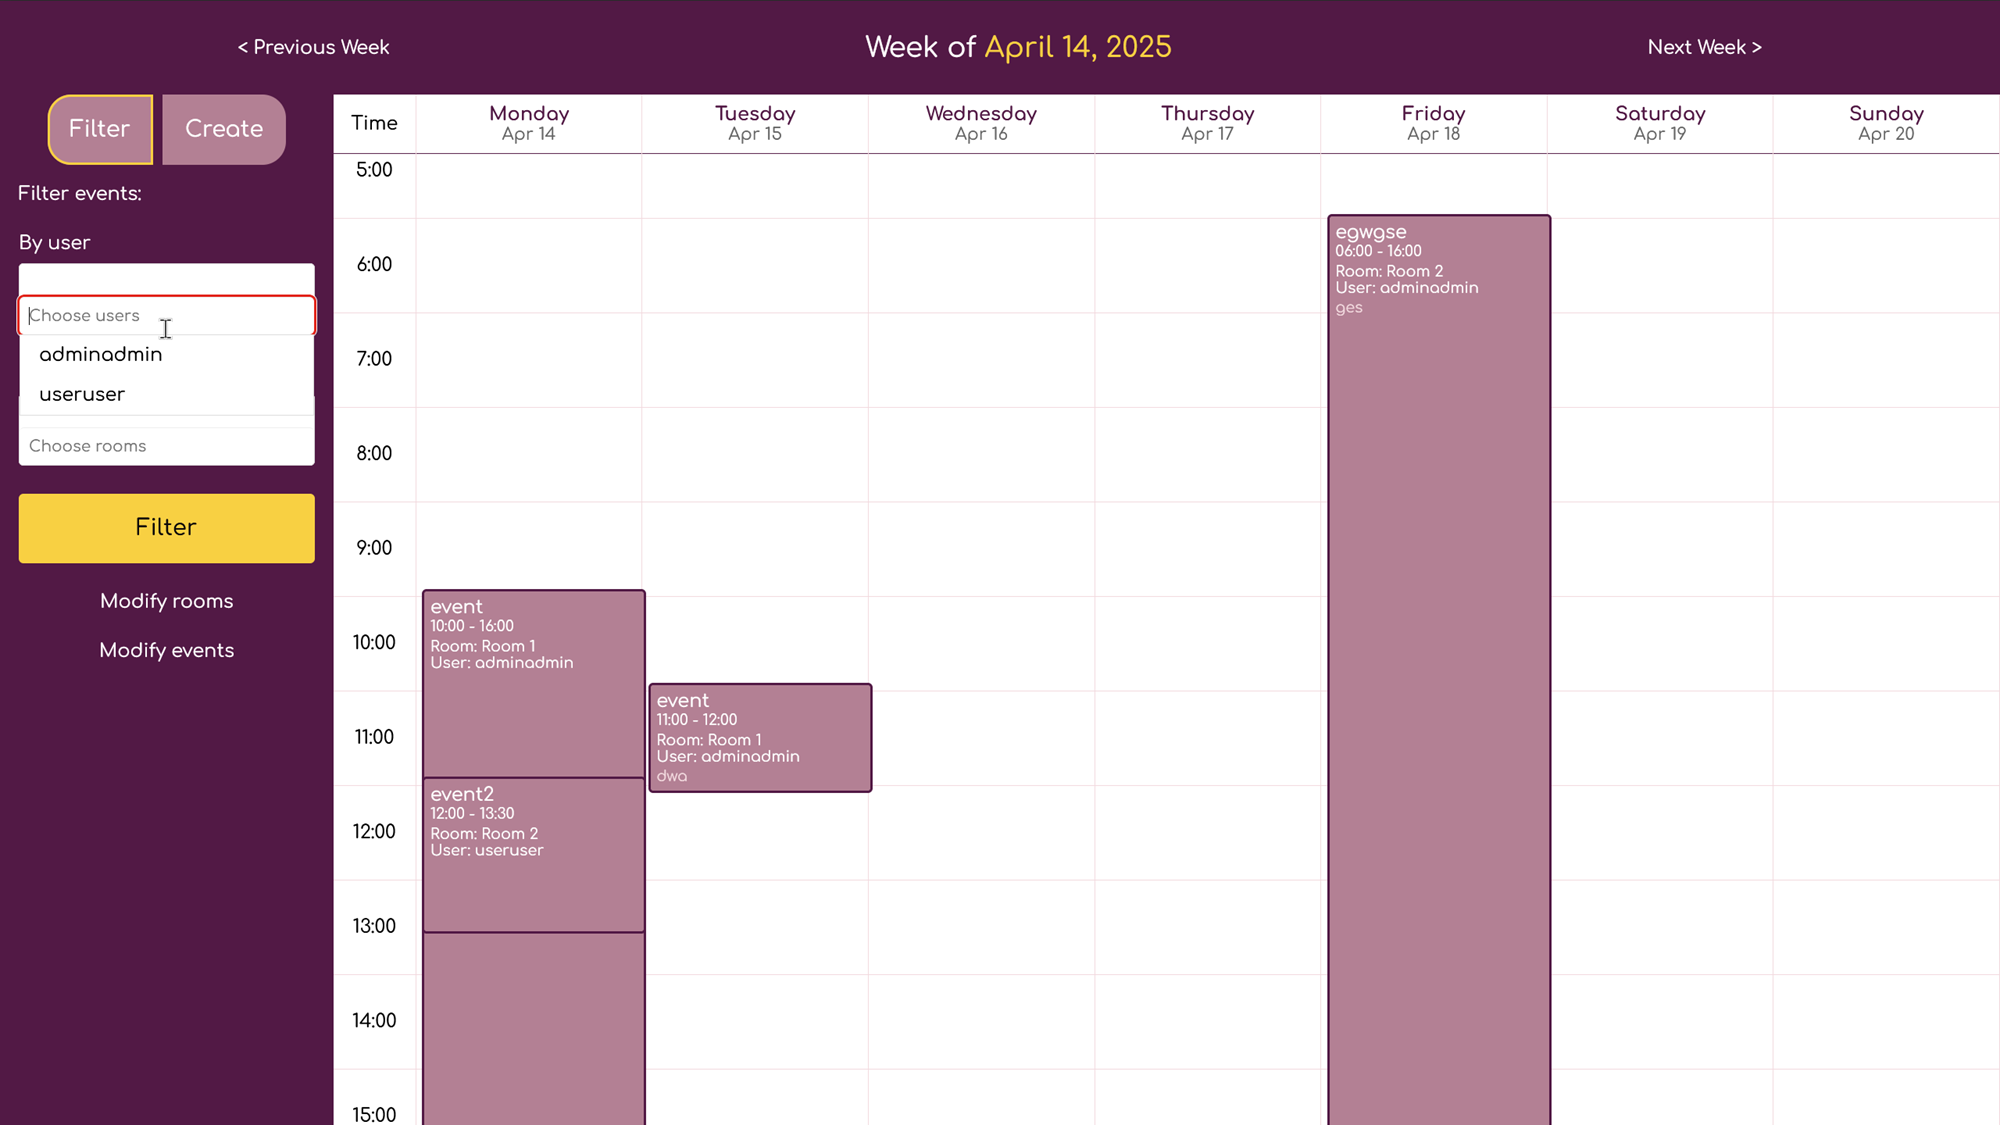
\includegraphics[width=0.6\textwidth]{TeamJob}
  \caption{Screenshot of the new solution}
  \label{fig:TeamJob}
\end{figure}
TeamJob is a web application that allows users to filter exactly what they want to see.
By default, all the events that are happening this week are shown.
The user can filter the events by the room and the person that is assigned to this event.
This allows for a more precise view of the calendar, where the user can see only the events that are important to them.
The user can also move between weeks.
A specific day-view allows the user to see the events that are happening on a specific day, if there are too many events to show them all at once.




    \chapter{Tools}\label{ch:tools}
    \section{Tool Selection and Technology Stack}\label{sec:tools}

This chapter examines the decision-making process behind selecting the technologies and tools for the team-work organization system.
The selection criteria were based on several key factors: project requirements, scalability needs, security considerations, and long-term maintainability.

\subsection{Framework Selection}\label{subsec:framework-selection}

Given the project's requirement to develop a Java application, the framework selection was focused on Java-based solutions.
The primary options considered were \textit{The Spring Framework}, \textit{Spring Boot},  \textit{Jakarta EE} (formerly Java EE), and \textit{Micronaut}.
Although all of these frameworks are capable of building robust web applications, they differ significantly in their approach and complexity.

\textbf{Jakarta EE}, the enterprise edition of Java, provides a comprehensive set of specifications to build enterprise applications.
However, it requires significant boilerplate code and configuration, making it less suitable for this project.
\textbf{Micronaut}, while promising with its ahead-of-time compilation and low memory footprint, is relatively new and has a smaller community compared to Spring Boot.

\textbf{The Spring Framework}, the foundation of Spring Boot, is a comprehensive programming and configuration model for modern Java-based enterprise applications.
It provides a wide range of features including dependency injection, aspect-oriented programming, and transaction management.
However, the Spring Framework requires extensive configuration and setup, which can be time consuming and complex.

\textbf{Spring Boot}, built on top of the Spring Framework, was selected as it addresses these configuration challenges while maintaining all the benefits of the Spring Framework.
It provides the following:
\begin{itemize}
    \item Auto-configuration of Spring Framework components
    \item Embedded servers for simplified deployment
    \item Production-ready features like metrics and health checks
    \item Reduced boilerplate code and configuration
\end{itemize}

This combination of Spring Framework's robust features and Spring Boot's simplified development approach makes it ideal for this project.
The framework's extensive documentation, large community support, and proven track record in enterprise applications further reinforce this choice.

\subsection{Frontend Technology Selection}\label{subsec:frontend-selection}

The selection of front-end technology required careful consideration of integration capabilities with Spring Boot.
\textbf{Thymeleaf}, as a server-side template rendering engine, was identified as the preferred option due to several factors.
It utilizes server-side page rendering to decrease the computational load on client systems.
Its integration of Java with HTML makes it relatively straightforward to use.
Furthermore, it is frequently used in conjunction with the Spring Boot.
Although modern alternatives like \textbf{React} and other JavaScript frameworks are prevalent, they would require significant additional research and development time.

The decision to use Thymeleaf was influenced by the simplicity of combining HTML and Java code in a single file.
However, modern web development requirements necessitated the incorporation of some JavaScript for specific client-side tasks, particularly for handling asynchronous requests and dynamic content updates.

\subsection{Database Selection}\label{subsec:database-selection}

\textbf{PostgreSQL} was selected as the primary database system after evaluating various database options, including NoSQL alternatives.
This choice was driven by PostgreSQL's prevalence in the market and its robust ACID compliance, which ensures data integrity and reliability.
The ACID properties provide essential guarantees for data management:

\begin{itemize}
    \item \textbf{Atomicity}: Ensures transactions are completed entirely or not at all.
    \item \textbf{Consistency}: Maintains database validity through all transactions.
    \item \textbf{Isolation}: Prevents concurrent transactions from interfering with each other.
    \item \textbf{Durability}: Guarantees committed transactions remain permanent.
\end{itemize}

These properties are crucial for maintaining data integrity in a multi-user environment where concurrent access and modifications are common.

\subsection{Security Architecture Decisions}\label{subsec:security-decisions}

The security implementation strategy was developed after careful analysis of the security requirements of modern web applications.
The decision to use \textbf{JWT-based authentication} was made after considering several factors, including the benefits of a stateless architecture that eliminates server-side session storage and improves scalability.
The approach also offers excellent cross-platform compatibility, enabling seamless integration with various clients while maintaining compliance with industry best practices for web security.
Alternative approaches like \textbf{session-based authentication} were evaluated but rejected due to their increased complexity with server-side session storage, increased server resource requirements, and complex session management.


The main security framework used is \textbf{Spring Security}, which provides a comprehensive security solution for Spring-based applications.
Although it is a powerful framework, it is not without its own challenges, such as the need to configure multiple security components and the potential for increased complexity in the codebase.
Still, the benefits of using a well-established security framework benefits the project in the long run.

\subsection{Development Tool Selection}\label{subsec:tool-selection}

The choice of development tools was guided by the need to improve code quality and development efficiency.
\textbf{Lombok} was selected because it effectively reduces boilerplate code without runtime overhead, integrates seamlessly with existing IDEs, and maintains code readability while reducing verbosity.
The IDE used is \textbf{IntelliJ IDEA}, which has excellent support for Java.

\subsection{Containerization Strategy}\label{subsec:containerization}

Containerization was implemented using \textbf{Docker} to ensure consistent deployment across different environments and simplify the development workflow.
The containerization strategy employs a multi-stage build process that optimizes both build time and final image size.
The build process utilizes \textbf{Amazon Corretto JDK 21} to compile the application and run it in a separate dockerfile stage.
The system includes integrated health checks to monitor container status, ensuring reliable operation and quick detection of potential problems.

This containerization approach delivers significant benefits to the project.
It ensures a consistent runtime environment across development, testing, and production stages, eliminating environment-specific issues.
The deployment process is simplified, reducing the complexity of moving the application between different environments.
Container isolation provides an additional layer of security, while the standardized container format enables easy scalability and orchestration capabilities.
Furthermore, this approach effectively eliminates the common ``works on my machine'' problem, as all environments run the same containerized application.
The basics of this approach were learned from the video resource~\cite{LearnDocker}.

\subsection{Technology Stack Integration}\label{subsec:integration}

The selected technologies were tested for their ability to work together.
The integration strategy focused on ensuring compatibility between all components, maintaining optimal system performance across all layers, and creating a system that can be easily updated and modified.
This careful selection and integration of technologies has resulted in a robust, scalable, and maintainable system that meets project requirements while providing a solid foundation for future enhancements.



    \chapter{Methods}\label{ch:methods}
    \section{Requirements Specification}\label{sec:requirements-specification}

\subsection{Functional Requirements}\label{subsec:functional-requirements}
The system provides comprehensive functionality in three main areas: \textbf{Basic Calendar Features}, \textbf{Additional Calendar Features}, \textbf{Secure Interactions}.

Under the \textbf{Basic Calendar Features} category, the system offers weekly and daily views, with filtering capabilities by room and user.
The system allows managers to create, edit, and delete events, while users can only view the calendar and search for resource availability.

In the \textbf{Additional Calendar Features} category, the system offers a day view, which displays events for a specific day organized by room.
Furthermore, the system offers a \texttt{FindAvailable} feature, which allows users to search for available resources (rooms, users, or events) based on various criteria.

Under the \textbf{Secure Interactions} category, the system offers a login system, which allows users to log into the system using a username and password.
The system stores all passwords in a hashed format using the BCrypt algorithm.
Instead of traditional session-based authentication, the system uses JWT tokens to authenticate users stateless-way.
This method was learned from the video resource~\cite{Amigoscode2023}.

\subsection{Non-Functional Requirements}\label{subsec:non-functional-requirements}

The application prioritizes function over design by providing a simple and intuitive user interface.
Navigation and interaction patterns remain consistent throughout the system, with clear error messages and feedback mechanisms to guide users.

Security is implemented through JWT-based authentication, with all communication restricted to HTTPS. The system incorporates protection against common web vulnerabilities and maintains strict access controls.

Reliability is ensured through robust error handling and data consistency mechanisms.

Maintainability is supported by comprehensive documentation, a modular architecture, and extensive test coverage.
This ensures that the system can be easily updated and maintained over time.


\section{System Architecture}\label{sec:system-architecture}

\subsection{Overall Architecture}\label{subsec:overall-architecture}
The application follows a four-tier architecture pattern, separating concerns across \texttt{Models}, \texttt{Views}, \texttt{Controllers}, and the \texttt{Database}. This separation enables better maintainability and scalability while keeping the system modular and efficient.
(See fig.~\ref{fig:architecture} for the system architecture diagram.)

\begin{figure}[h]
    \centering
    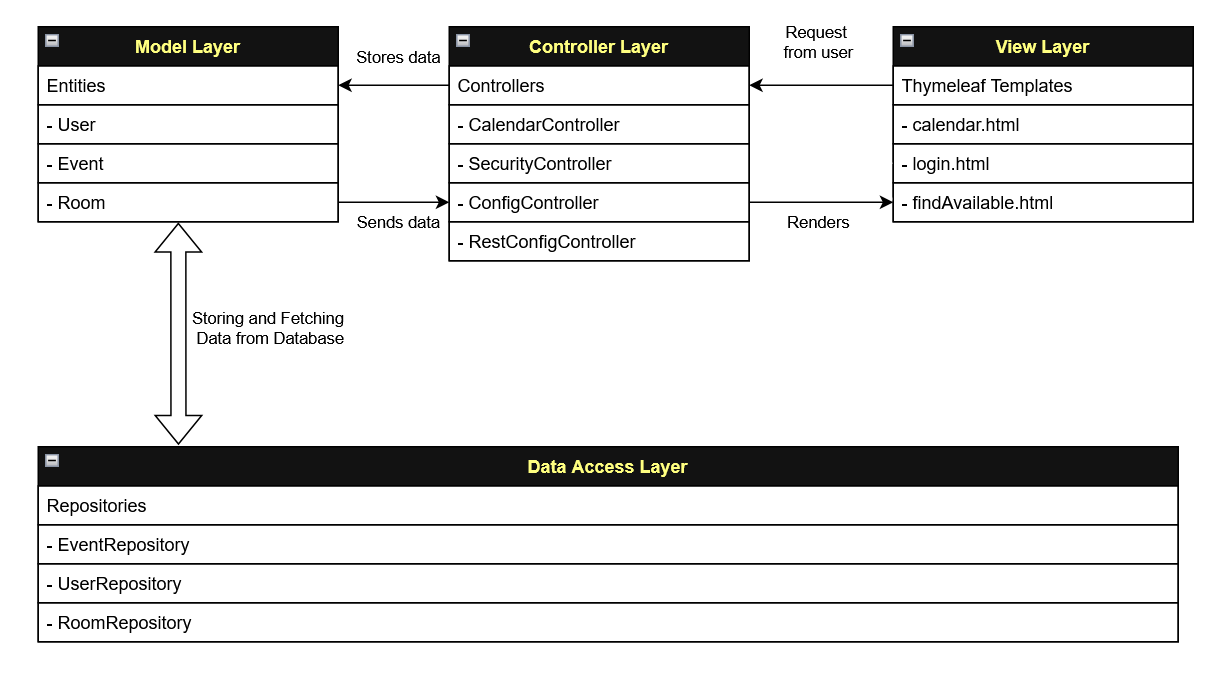
\includegraphics[width=0.8\textwidth]{MVCSchema}
    \caption{System Architecture Diagram}
    \label{fig:architecture}
\end{figure}

\subsection{Key Components}\label{subsec:key-components}

The front-end components utilize Thymeleaf templates for server-side rendering, enhanced with JavaScript for client-side interactivity and CSS for design.
This combination provides a modern, dynamic user experience while maintaining performance, as the Thymeleaf templates are rendered on the server side.

The backend architecture consists of controllers handling HTTP requests and responses, services implementing business logic, repositories managing data access, and a comprehensive security layer handling authentication and authorization.

\subsection{API Design}\label{subsec:api-design}

The application provides both REST API endpoints and view-based endpoints to support various client needs.
The REST API follows standard conventions and provides endpoints for authentication, resource management, and system queries.

Authentication endpoints handle user sign-in, registration, and logout operations.
Resource endpoints manage rooms and events, while query endpoints provide functionality to check resource availability and validate authentication tokens.

View endpoints serve the user interface, with dedicated routes for calendar views and system configuration.
Calendar views support weekly and daily perspectives, while configuration views provide interfaces for managing rooms, events, and users.

The basics of this design were adopted following guidance from the video resource

~\cite{VisualComputerScience2023}.


\section{Database Design}\label{sec:database-design}

\subsection{Database Schema}\label{subsec:database-schema}
The database schema (see fig.~\ref{fig:schemaDB}) is designed around three main entities: users, rooms, and events.

After that, the \texttt{roles} table is used to manage the user roles.

In addition, 3 tables of \texttt{tags} are used to manage the tags for rooms, events, and users to simplify the search for resources.

\begin{figure}[h]
    \centering
    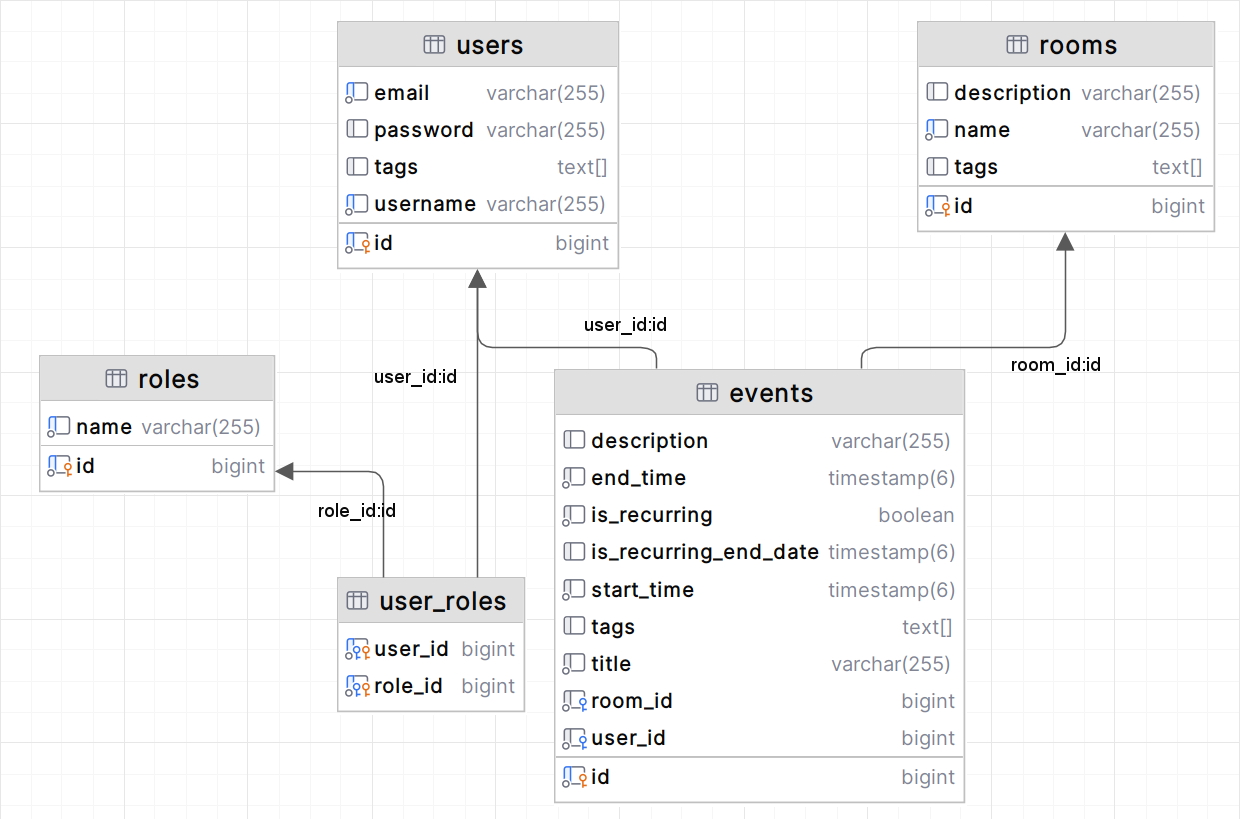
\includegraphics[width=1\textwidth]{schemaDB}
    \caption{Database Schema Diagram}
    \label{fig:schemaDB}
\end{figure}

\subsection{Key Tables and Relationships}\label{subsec:key-tables}

The table ``users'' stores essential user information, including username, email, and securely hashed passwords.
Maintains a many-to-many relationship with the role table, enabling flexible role assignment and management.
This solution is not the most elegant one, as it requires additional queries to get the roles of a user.
However, it was chosen to simplify the implementation of authentication(which validates permissions) and authorization(which validates access to resources).


The roles table defines the various user roles within the system, with a connection to the users table using another table called \texttt{user\_roles}.
This design allows for the easy addition of new roles and modification of existing role permissions.

The room table contains information about spaces, including names, descriptions, and categorization tags.
Creating a one-to-many relationship with the events table, the rooms table can have multiple events, but not at the same time.

The event table serves as the central scheduling entity, storing event details such as title, description, timing information, and recurrence settings.
Events maintain relationships with both users and rooms, tracking who is involved and where the event takes place.
Recurrence is implemented following the RFC 5545 standard\cite{rfc5545}.

\subsection{Spring Data JPA Implementation}\label{subsec:spring-data-jpa}

The application relies on Spring Data JPA for efficient data persistence.
Entity classes are annotated with @Entity and @Table, while repositories extend JpaRepository to provide standard CRUD operations.
Relationships between entities are managed through JPA annotations and Spring handles transaction management automatically.
The method of implementing the relationships was learned from the spring.io wiki~\cite{SpringDataJPA2024}.


\section{User Interface Design}\label{sec:ui-design}

\subsection{Design Philosophy}\label{subsec:design-philosophy}
The design of the user interface emphasizes simplicity, consistency, responsiveness, and accessibility.


% Converted HSL→RGB→hex (approximate)
\definecolor{colorGold}{HTML}{F9E14D}       % from HSL(46.8,92.9,61.6)
\definecolor{colorSecondary}{HTML}{C78094}  % HSL(336,25,60)
\definecolor{colorTertiary}{HTML}{772852}   % HSL(314,53,21)
\definecolor{colorAccent}{HTML}{662640}     % HSL(339,27,17)
\definecolor{colorAdditional}{HTML}{0B0A0A}% HSL(345,18,4)

The main colors are
\begin{itemize}
    \item \textcolor{colorGold}{\textbf{--color-gold} (46.8\%, 92.9\%, 61.6\%): Gold}
    \item \textbf{--color-primary} (0\%, 0\%, 100\%): White
    \item \textcolor{colorSecondary}{\textbf{--color-secondary} (336\%, 25\%, 60\%): Dusty Rose}
    \item \textcolor{colorTertiary}{\textbf{--color-tertiary} (314\%, 53\%, 21\%): Deep Magenta}
    \item \textcolor{colorAccent}{\textbf{--color-accent} (339\%, 27\%, 17\%): Plum}
    \item \textcolor{colorAdditional}{\textbf{--color-additional} (345\%, 18\%, 4\%): Charcoal}
\end{itemize}

\subsection{Key Interface Components}\label{subsec:interface-components}

The calendar view presents a weekly grid layout with color-coded events.

Event management features include forms to create and edit events, quick filters for different event types, and clear conflict warnings.
The interface guides users through the event creation process while preventing scheduling conflicts.

Navigation is streamlined through a consistent menu structure.



    \chapter{Results}\label{ch:results}
    \section{Calendar Interface and Rendering}\label{sec:calendar-interface-and-rendering}
The calendar is the primary interface of the application, implemented through an integration of Thymeleaf templates and JavaScript to enhance interactivity.
The underlying backend functionality is administered by the CalendarController and CalendarServiceImpl service.
Upon users' access to the calendar, the controller delegates service methods such as setupModelForWeekCalendar and setupModelForDayCalendar to the responsibility of preparing the required data for the rendering of weekly or daily views.
These methods retrieve all pertinent events from the database, filter them according to user, room, and tag parameters, and structure them into entities such as WeekDay and EventInADay.
The filtration process is thorough, accommodating combinations of user IDs, room IDs, and tags, and is implemented in the service layer through the use of helper methods that parse and apply these filters.
Subsequently, the calendar view is rendered by Thymeleaf, which receives all data as model attributes, while JavaScript is employed to augment navigation and interactivity, easing shifts between weeks or days.


\section{Event Creation, Validation, and Conflict Detection}\label{sec:event-creation-validation-and-conflict-detection}
The creation of events is managed through REST endpoints within the RestConfigController.
Upon submission of a new event by the user, the backend initiates a check for scheduling conflicts employing the findOverlappingEventsInRoom method of the EventRepository.
This mechanism ensures that no two events simultaneously occupy the same room.
In instances where a scheduling conflict is identified, the system issues a conflict response, requiring the user to select an alternative time or resource.
The event creation process accommodates both singular and recurring events.
For recurring events, the system constructs an RRULE string that complies with RFC 5545 standards, including support for intervals, end dates, and specific weekdays in the case of weekly recurrences.
The event entity is responsible for maintaining all recurrence-related information, including exception dates (exdate) and supplementary dates (rdate).
While the backend logic for recurring events is fully implemented and functional, the frontend display of recurring events in the calendar interface has not been completed.
The system successfully stores and processes recurring event data, but the visual representation of these events in the calendar views requires further development.
In addition, the DefaultValueService has been implemented to facilitate the demonstration of the project.
It generates test events, users, and rooms to verify the system's functionality under conditions of load.


\section{Filtering by User, Room, and Tags}\label{sec:filtering-by-user-room-and-tags}
The capability to filter is a fundamental aspect of the calendar and event views.
The backend enables the filtration of events based on user IDs, room IDs, and tags associated with users, rooms, or events.
This functionality is executed in the CalendarServiceImpl service, where methods such as convertToDayEvents and generateAvailableTimeRequest implement filters on the event list prior to rendering to the frontend.
The filtering mechanism interprets comma-delimited strings of IDs or tags, converts these into sets, and applies them to the event data using Java Streams and supporting techniques.
Consequently, events are excluded if their associated user, room, or tags do not correspond to the designated criteria.
This enables users to focus on the most relevant events, even in scenarios marked by a substantial number of planned activities.


\section{Authentication and Role-Based Access Control}\label{sec:authentication-and-role-based-access-control}
Authentication is achieved through the use of JWT (JSON Web Tokens), with the SecurityController overseeing the workflows of sign-in, sign-up, and sign-out.
The user credentials are subjected to secure hashing and storage, and the JWT tokens are distributed upon successful completion of authentication.
The TokenFilter plays a critical role in intercepting requests, extracting and validating JWT tokens, and establishing the security context for the authenticated user.

Role-based access control is enforced throughout the application.
Users are assigned specific roles such as ROLE\_USER, ROLE\_ADMIN, or ROLE\_CONFIG, which are stored within the database and linked to each user.
The SecurityConfigurator utilizes Spring Security to impose access restrictions on sensitive endpoints that depend on these roles.
For instance, only users possessing roles of ROLE\_CONFIG or ROLE\_ADMIN are authorized to create, edit, or delete events and rooms, whereas regular users are restricted to activities like viewing and searching.
CSRF protection is systematically enabled for all forms.

The auditing part of the Spring Data framework\cite{AuditingSpringData} serves as a mechanism to monitor alterations to entities.
It records the timestamp of creation, identifies the creator, and documents the identity and timing of modifications within the database.
This framework facilitates the verification of the authorship of any modifications made within the system.


\section{Tagging System}\label{sec:tagging-system}
The application incorporates a robust tagging system applicable to users, rooms, and events.
Tags are maintained as collections of strings within each entity (User, Room, Event) and are stored in separate tables utilizing JPA's @ElementCollection.
Tags are employed extensively throughout the interface for the purposes of filtering and searching, and are also presented in both list and detailed views.
The backend includes methods to retrieve all unique tags from the database, which are subsequently displayed in dropdown menus and filter panels within the user interface.
Tag-based filtering is executed within the service layer, enabling users to efficiently access pertinent information by selecting one or more tags.
Furthermore, the system supports the allocation of random tags to entities during the generation of test data, thus ensuring a diverse array of tags for both demonstration and testing purposes.


\section{Error Handling and Custom Error Pages}\label{sec:errorHandlingAndCustomErrorPages}
The management of errors is facilitated by an error controller, referred to as the CustomErrorController, which intercepts errors and generates a comprehensive error page \texttt{error-debug.html}.
This controller is responsible for extracting error statuses, exception details, messages, and the pathways of requests, and it incorporates stack traces whenever they are available.
This methodology affords developers and administrators exhaustive information necessary for debugging and system maintenance, while concurrently supplying end users with lucid feedback regarding any issues encountered.


\section{Room and User Management}\label{sec:roomAndUserManagement}
The management of rooms and users is integrated into both backend and frontend systems.
The ConfigController offers endpoints for the enumeration, addition, and removal of rooms and users.
In the backend, there are strict verifications to ensure that only users with designated roles are authorized to carry out these operations.
The system performs checks to ensure uniqueness in identifiers such as room name, username, and email.

The frontend displays comprehensive lists of rooms and users, inclusive of their tags and roles, and provides forms for the entry of new data.
The deletion process is secured by the inclusion of confirmation prompts and backend verifications to avert the inadvertent removal of critical resources.
Additionally, the system accommodates the bulk management of events, rooms, and users, thereby enhancing the efficiency of administrative functions.


\section{Find Available Functionality}\label{sec:findAvailableFunctionality}
The ``Find Available'' functionality is executed within the CalendarController and CalendarServiceImpl.
Users are enabled to query for available rooms or users by specifying relevant tags, date, start, and end times, as well as the desired duration.
The backend systematically processes these inputs, computes unoccupied time slots using the generateAvailableTimeRequest method, and subsequently provides a list of available resources.
The returned results include direct links to observe availability within the calendar, thus significantly streamlining the scheduling of meetings or events in environments characterized by high demand for bookings.
This particular functionality is notably absent from the existing scheduling system implemented at my University.

\newpage
\section{Installation and Deployment tutorial}\label{sec:installationAndDeploymentTutorial}
The installation of this project was made simple and straightforward.

\textbf{Firstly, install docker.} This can be done either from the official website or from the package manager of your operating system.
For example, on Ubuntu, you can install docker using the following commands (From the official website~\cite{DockerWebsite}):
\begin{minted}{bash}
sudo apt-get update
sudo apt-get install ca-certificates curl
sudo install -m 0755 -d /etc/apt/keyrings
sudo curl -fsSL https://download.docker.com/linux/ubuntu/gpg -o /etc/apt/keyrings/docker.asc
sudo chmod a+r /etc/apt/keyrings/docker.asc

echo \
 "deb [arch=$(dpkg --print-architecture) signed-by=/etc/apt/keyrings/docker.asc] https://download.docker.com/linux/ubuntu \
 $(. /etc/os-release && echo "${UBUNTU_CODENAME:-$VERSION_CODENAME}") stable" | \
 sudo tee /etc/apt/sources.list.d/docker.list > /dev/null
sudo apt-get update

sudo apt-get install docker-ce docker-ce-cli containerd.io docker-buildx-plugin docker-compose-plugin git
\end{minted}
This will install git, docker and docker-compose.

\textit{Note:} If you are using a different operating system, you can find the installation instructions on the official website.

\textbf{Secondly, clone the repository.} This will be done using git that was installed in the previous step.
\begin{minted}{bash}
git clone https://github.com/KirillBorodinskiy/TeamJob.git
\end{minted}

\textbf{Thirdly, build and run the project.} This will be done using docker-compose that was pre-configured to handle all tasks and dependencies automatically.
\begin{minted}{bash}
cd TeamJob
docker-compose up
\end{minted}

The application will be accessible through a web browser at \url{http://localhost:8080} upon successful deployment.
The default port configuration can be modified within the \texttt{docker-compose.yml} file to accommodate specific network requirements or port conflicts.
This containerized deployment approach ensures consistent execution environments across different operating systems and eliminates the need for manual dependency management.

For development and customization purposes, the application can be executed without Docker containerization, though this approach necessitates additional configuration and setup procedures.
This alternative deployment method requires the installation of Java Development Kit (JDK) version 21, which can be obtained from the official Oracle website or through package managers such as Homebrew on macOS or apt on Ubuntu systems.
The local execution process involves navigating to the project directory and utilizing the Gradle wrapper to compile and run the application:

\begin{minted}{bash}
cd TeamJob
./gradlew build
\end{minted}

This non-containerized approach requires manual configuration of the PostgreSQL database, including the establishment of database credentials, creation of the database instance, and configuration of connection parameters within the application properties.
Additionally, users must ensure that all required environment variables are properly set, including database connection strings, authentication secrets, and application-specific configurations.
This deployment method is particularly suitable for developers who require direct access to the application source code for customization, debugging, or integration with existing development workflows.

\newpage
\section{Usage tutorial}\label{sec:usageTutorial}
The application provides an intuitive and comprehensive user interface designed to facilitate efficient scheduling and resource management.
The system implements a multi-layered authentication mechanism and offers extensive functionality for calendar management, event creation, and administrative operations.

\textbf{The authentication system} utilizes JSON Web Tokens (JWT) to facilitate secure session management throughout the application.
User registration is allowed through multiple endpoints (\texttt{/signup} and \texttt{/register}), with authentication processes available via \texttt{/login}, \texttt{/signin}, and the primary endpoint \texttt{/}.

This redundant routing approach ensures ease of access regardless of the user's point of entry.
Following successful authentication, the system issues a cryptographically secure JWT token, which is retained in the browser's cookie storage, providing persistent session management while upholding security through token expiration and validation.
The implementation includes comprehensive error handling mechanisms for invalid credentials and session expiration.

\textbf{The primary calendar interface} at \texttt{/calendar} functions as the central operational hub, allowing users to visualize, create, and manage events through an intuitive interface.
This interface accommodates both weekly and daily perspectives, allowing users to traverse different temporal views.

Detailed event information is accessible via the \texttt{/event/\{id\}} endpoint, which provides comprehensive data, including participant details, room allocations, and related metadata.
Information specific to rooms can be obtained through the \texttt{/room/\{id\}} endpoint, which provides extensive room specifications, availability patterns and organizational tags.

The centralization of \textbf{administrative functionality} is achieved via the hierarchy of the \texttt{/config} endpoint.
The \texttt{/config/rooms} endpoint provides capabilities for room management, facilitating administrators to view, create, and modify room configurations that include capacity specifications, equipment details, as well as organizational tags.
The \texttt{/config/events} endpoint provides event management functionality, including reviewing scheduled events, modifying event details, and managing event-specific metadata.
In addition, user management through \texttt{/config/users} grants administrative access to user account information, role assignments, and user-specific configurations.

This administrative interface supports role-based access control, allowing system administrators to allocate appropriate permissions and organizational roles.
The system employs comprehensive audit trails for all administrative operations, ensuring accountability and offering detailed logs for purposes related to security and compliance.

The \texttt{/calendar/findAvailable} endpoint enables the \textbf{identification of available resources} by allowing users to apply specific criteria such as temporal constraints, resource tags, and duration requirements.
This capability is particularly advantageous in contexts characterized by high resource contention, as it allows users to optimally identify appropriate time slots and resources.

In addition, the system offers extensive \textbf{filtering capabilities}, allowing users to concentrate on designated subsets of events and resources.
Users have the ability to filter calendar views based on user identifiers, room specifications, and organizational tags, creating personalized views that improve the salience of pertinent information while mitigating cognitive load.
The realization of this filtering functionality is facilitated through the integration of front-end interface controls alongside back-end query optimization processes; thus, it should maintain performance efficiency even while handling large datasets.



    \chapter{Discussion}\label{ch:discussion}
    The development of TeamJob represents a significant undertaking in modern web application development, but the project's true value lies not merely in its technical implementation, but in the insights it provides about software engineering practices, architectural decision-making, and the challenges of creating organizational tools.
This discussion critically examines the project's successes, limitations, and broader implications.


\section{Architectural Decisions and Their Implications}\label{sec:architectural-decisions-and-their-implications}

Spring Boot selected (Section~\ref{sec:technology-choices}); MVC structure clarified, service layer introduced (Section~\ref{sec:testing-strategy}); JWT authentication implemented (Section~\ref{sec:security-implementation}); calendar system designed for RFC 5545 (Section~\ref{sec:calendar-functionality}); PostgreSQL and H2 configured (Section~\ref{sec:database-design2}); Thymeleaf-based UI chosen (Section~\ref{sec:user-experience-/-user-design}); comprehensive testing applied (Section~\ref{sec:testing-strategy}); technology stack evaluated (Section~\ref{sec:technology-choices}).


\section{Security Implementation}\label{sec:security-implementation}

The implementation of JWT-based authentication represents a modern, state-less approach to authentication.
This was further intensified by the reluctance to manually manage sessions or establish a dedicated system for this purpose.
The issue of improper configuration of the filter chain has frequently emerged; however, with the current setup, such complications should no longer arise during application usage.

Another potential issue is the implementation of distinct account storage and logging systems.
This approach may not be compatible with organizations that employ a single account per individual across all their systems.
This challenge could be addressed by extensively modifying the source code, given that the program is entirely open to modification and redistribution.


\section{Calendar Functionality}\label{sec:calendar-functionality}

The calendar system represents the project's most complex component, and its implementation reveals both the power and limitations of the chosen approach.
The RFC 5545 compliance for recurring events, while technically correct in the backend implementation, introduced significant complexity that affected the frontend display development.
The availability calculation algorithms, while efficient for moderate datasets, may not scale to enterprise-level deployments with thousands of users and events.

The powerful filtering system offers users the ability to identify the most suitable schedule.
However, the challenge lies in the extensive filtering required.
An idea emerged later in the project to establish predefined tag groups tailored for specific student demographics, such as first-year students in the XYZ program.
Students would have the opportunity to adjust these tags to meet their specific requirements.
The implementation of this feature has been canceled due to time constraints.


\section{Database Design}\label{sec:database-design2}

Employing a PostgreSQL database within a Docker container was a strategically beneficial decision; however, it introduced a certain level of complexity when working within a local environment utilizing an H2 database.
Considerable time was devoted to the issues of \texttt{ application.properties} and \texttt{ application-test.properties}.
Eventually, the configuration was adapted to utilize the \texttt{.env} file for the deployed environment, while locally-selected variables were employed for test cases.

The current method for implementing the \texttt{ user\_roles} table and ``tags'' tables is functional.
However, it may ultimately complicate the comprehension of the entire system and its operational mechanics.

\newpage

\section{User Experience / User Design}\label{sec:user-experience-/-user-design}

The user interface design prioritizes functionality over aesthetics, which is appropriate for an organizational tool, but may limit adoption in environments where user experience is of the utmost importance.
The use of a Thymeleaf-based methodology ensures robust performance and security; however, it restricts the level of dynamic interactivity anticipated by modern users.
This limitation could be addressed by transitioning to the currently prevalent JavaScript frameworks.
However, the author lacked the requisite expertise in such frameworks, and temporal constraints precluded this transition.

\begin{figure}[htbp]
    \centering
    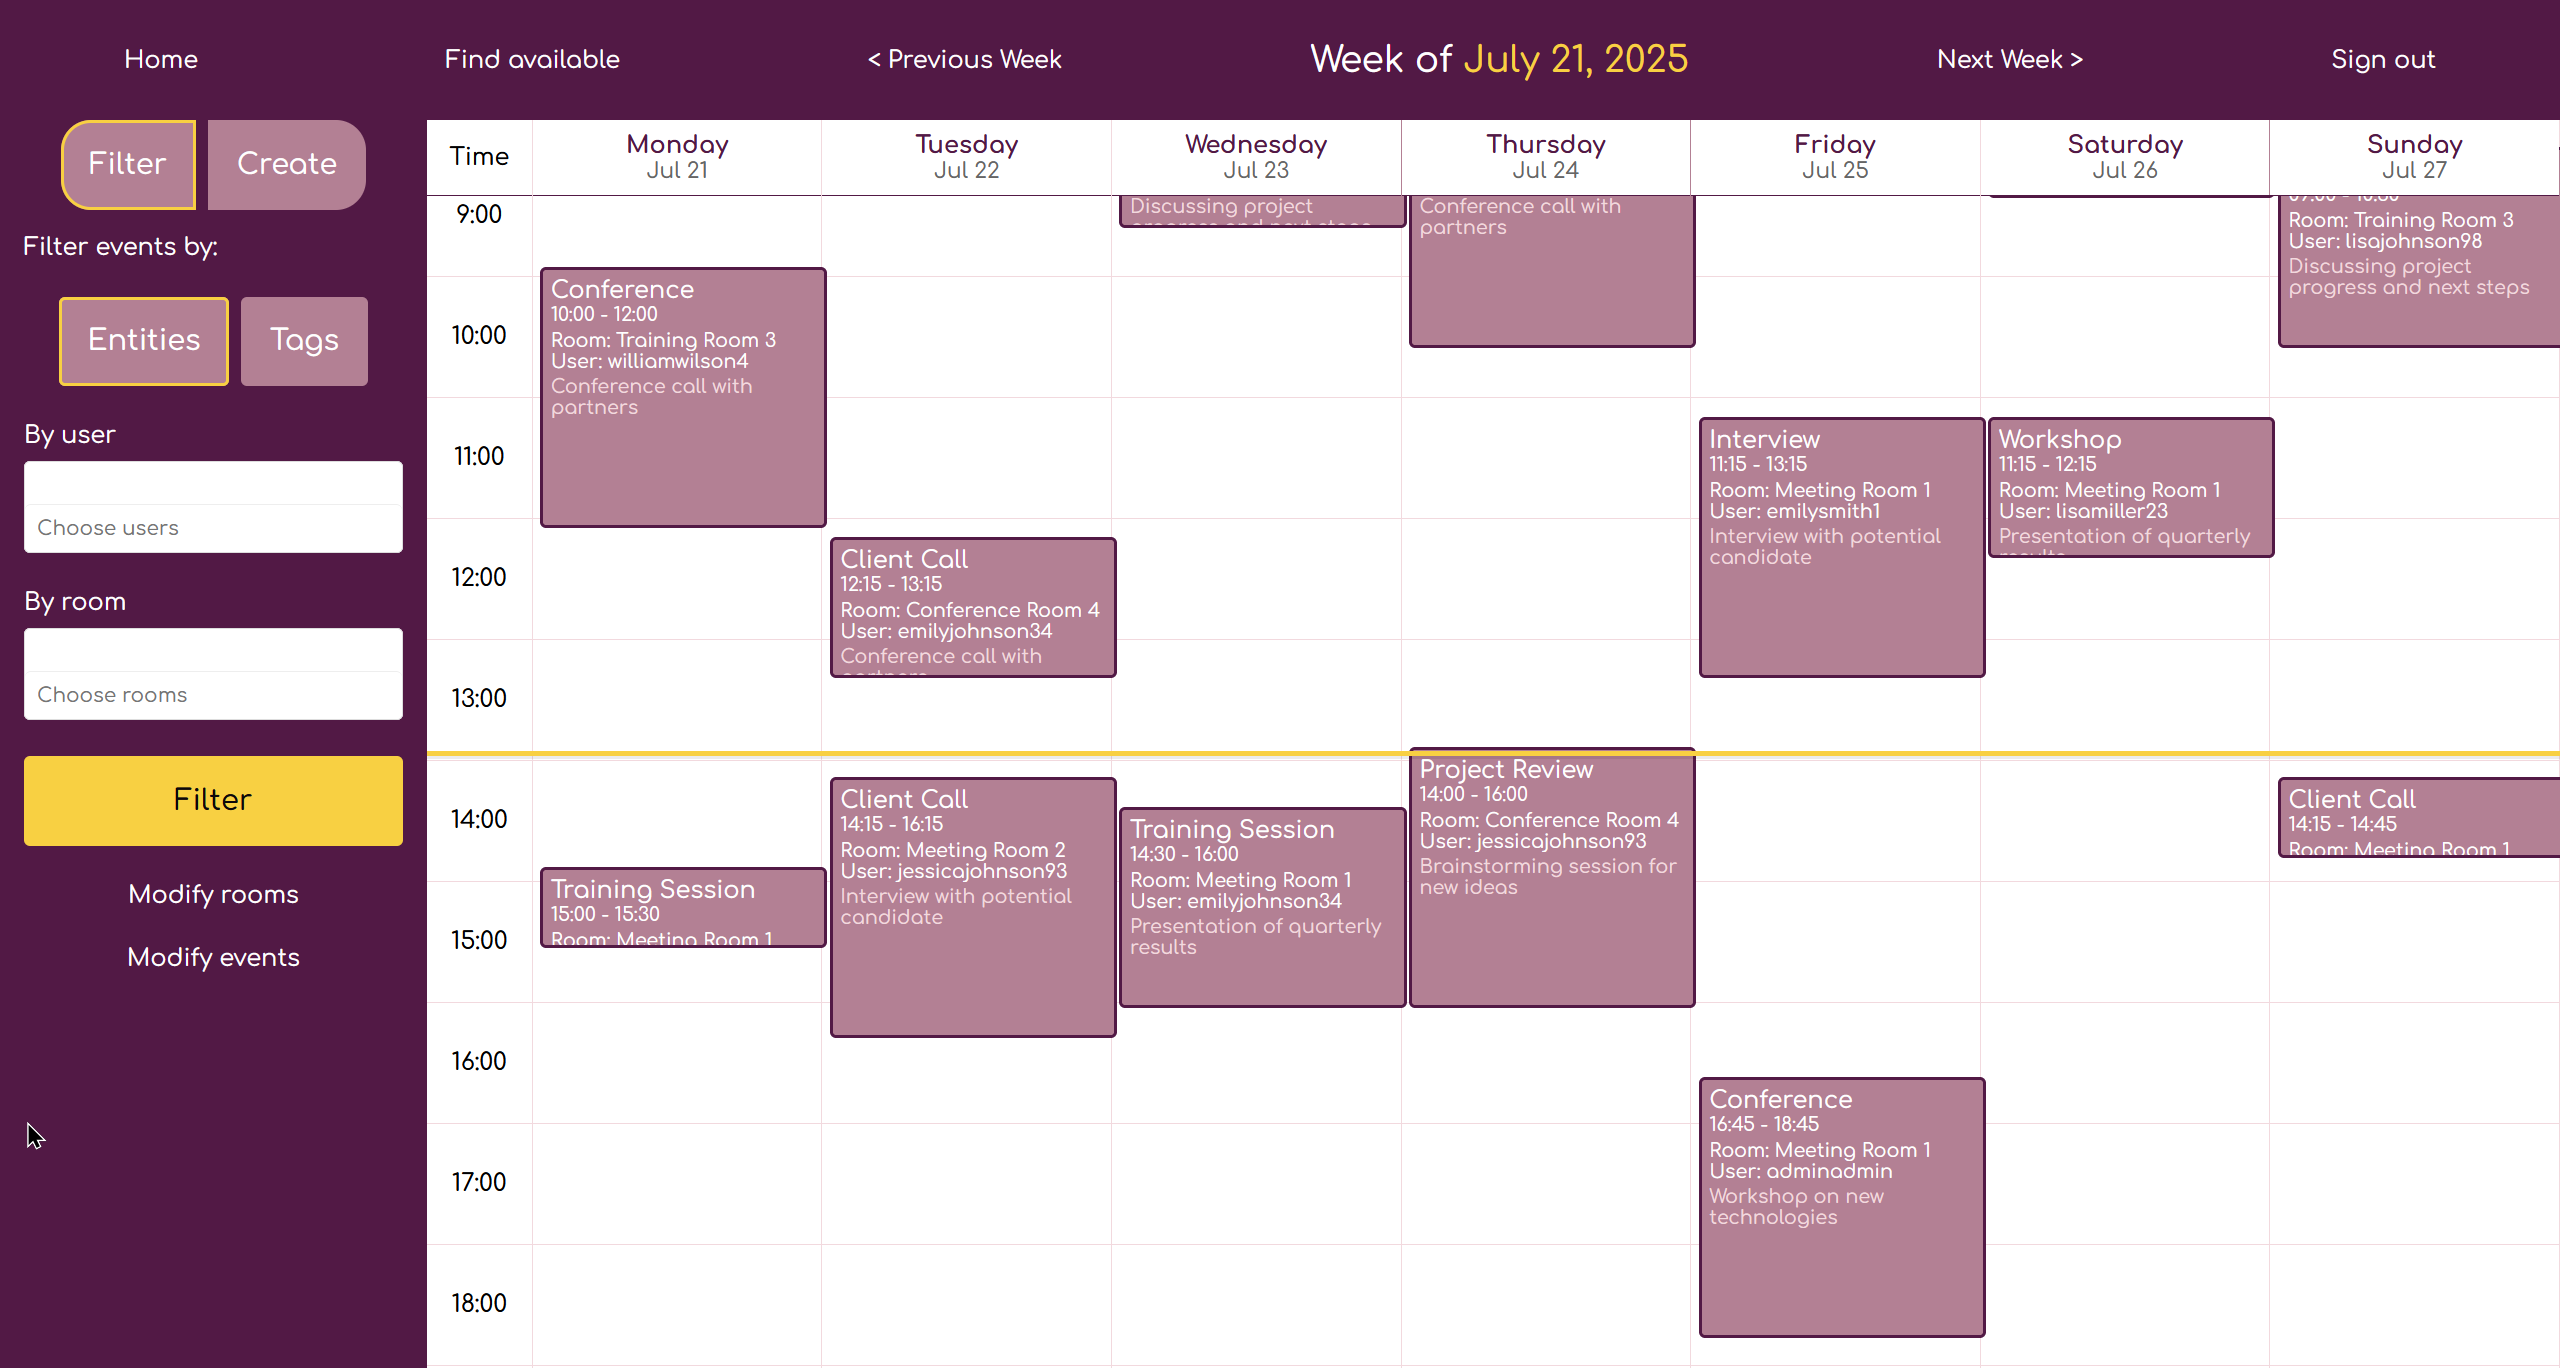
\includegraphics[width=0.8\textwidth]{Week_view}
    \caption{Weekly calendar view interface of the TeamJob application displaying scheduled events in a grid format.}
    \label{fig:week-view}
\end{figure}

The creation of an effective calendar interface presents the challenge of displaying scheduling data in a way that is both clear and user-friendly.
Feedback from an expert within the design domain has been positively received regarding the UI elements~\ref{fig:week-view} of the application, particularly applauding the selection of color schemes and the intuitive nature of the navigation system.


\section{Testing Strategy}\label{sec:testing-strategy}
The testing methodology employed within TeamJob was characterized by a comprehensive and detailed examination that included the service, controller, and repository layers.

\textbf{Test Data Management:} Each test class independently configures and dismantles its data to ensure both isolation and repeatability.
Helper methods are used to create realistic test entities, and the database is meticulously cleaned before and after each test to prevent cross-test contamination.

\textbf{Service Layer Testing:} The \texttt{CalendarServiceImplTest} class employs JUnit 5 and Mockito to thoroughly evaluate the business logic inherent in the calendar service.
The service logic is effectively isolated through the injection of mock repositories, and comprehensive test data is generated for users, rooms, and events.
The testing protocol covers various scenarios, such as event conversion, recurrence rules, filtering, and overlapping events, to verify that the core scheduling logic functions correctly.

\textbf{Controller Layer Testing:} The \texttt{RestConfigControllerTest} class employs Spring Boot's \texttt{@SpringBootTest} and \texttt{@AutoConfigureMockMvc} to execute integration testing on REST endpoints.
These assessments simulate authentic HTTP requests through the utilization of MockMvc, validating authentication, authorization, and accurate handling of event creation, including the backend processing of recurring events.
JWT tokens are systematically generated for a variety of user roles to evaluate access control mechanisms.
The validation procedures ensure that actions are executable exclusively by users with the necessary roles and that the API delivers precise responses to both legitimate and illegitimate requests.

\textbf{Repository Layer Testing:} The \texttt{EventRepositoryTest} and \texttt{RoomRepositoryTest} classes utilize \texttt{@DataJpaTest} to assess the persistence layer through an in-memory database.
Validates custom query methods designed to locate events based on time, room, title, and tags, as well as to detect overlapping events.
These tests verify the precision of the repository logic and the ability of the database schema to facilitate the necessary queries.

\begin{table}[htbp]
    \centering
    \caption{Test Suite Results Summary}
    \begin{tabular}{|p{0.5\textwidth}|c|}
        \hline
        \textbf{Test Category}    & \textbf{Pass Rate}     \\
        \hline
        Application Context Tests & 100\% (1/1)            \\
        \hline
        Controller Tests          & 100\% (9/9)            \\
        \hline
        Repository Tests          & 100\% (12/12)          \\
        \hline
        Service Tests             & 100\% (25/25)          \\
        \hline
        \textbf{Total}            & \textbf{100\% (47/47)} \\
        \hline
    \end{tabular}
    \label{tab:test-results}
\end{table}


\section{Technology Choices}\label{sec:technology-choices}

The technology stack represents a solid choice for the project requirements, but each component introduces both benefits and trade-offs.
Spring Boot eases developer productivity and offers a wide array of extensions along with support for various features.
Despite its extensive customization capabilities, alternative back-end frameworks may present configuration options that are more straightforward.
PostgreSQL is the highly popular database for modern applications.
It is often used for both small-scale applications and enterprise applications.\cite{ThebenefitsofPostgreSQL,GerritMeyer2025}

The use of Thymeleaf as a templating engine guarantees substantial security and performance.
However, it limits the dynamic user experience that is often required by modern applications.
In contrast, contemporary JavaScript frameworks enable the development of more dynamic pages, facilitating easier reuse of design patterns and additional features.



    \chapter{Conclusion}\label{ch:conclusion}
    This thesis aimed to design and implement a self-hosted, open-source team scheduling system specifically suited for organizations that prioritize privacy, flexibility, and control over their scheduling data.
Through an analysis of existing solutions and their associated limitations, the project defined clear objectives:
design a user-friendly, customizable, and secure calendar application that employs modern Java web technologies and has necessary features for a team scheduling system.

The selection of Spring Boot, Thymeleaf, and PostgreSQL provided a robust foundation, effectively balancing ease of development, security, and scalability.
The implementation adhered to best practices in software architecture, using a modular MVC pattern and integrating JWT-based authentication to ensure secure stateless user sessions.
The resultant system offers a comprehensive suite of features, including advanced event management, conflict detection, filtering, and a flexible tagging system, all accessible via an intuitive Web interface.

Extensive testing at the service, controller and repository levels confirmed the reliability and correctness of the system.
The project's discussion underscored both the strengths and trade-offs of the selected technologies, as well as the challenges encountered in areas such as:
\begin{itemize}
    \item UI interactivity,
    \item Database configuration,
    \item Recurring event logic.
\end{itemize}
The successful attainment of these objectives yielded several significant outcomes.
Primarily, the project facilitated a comprehensive understanding of Java web development libraries and their practical applications, realized through the evaluation, selection, and integration of technologies including Spring Boot, Thymeleaf, and PostgreSQL\@.

The outcome is a functional application designed for team work organization, enabling efficient team collaboration, providing intuitive event management, ensuring secure system interactions, and offering a responsive and user-friendly interface.

Furthermore, the project created detailed documentation covering the technology evaluation and selection process, system architecture and design decisions, implementation specifics, testing methodology, and results, which serves as an essential reference for subsequent development and analogous endeavors.

Finally, the project provided practical experience in Java web application development, database design and implementation, user interface development, and system testing and validation, thus improving both technical proficiency and project management abilities.

Although the application achieves its primary objectives, certain limitations persist.
The user interface, although functional, could benefit from enhanced dynamism and modern design patterns.
Scalability for very large organizations and further automation in tag management present opportunities for future enhancement.
In addition, integration with external authentication systems and the adoption of more interactive front-end frameworks could further enhance usability and adoption.

In conclusion, this work exemplifies the feasibility and value of a customizable, privacy-focused scheduling platform for organizations.
It provides a solid technical foundation and practical insights for future development, contributing both a functional solution and a reference point for similar ventures in the domain of collaborative scheduling systems.

    \printbibliography[title=Bibliography]

\end{document}
